\subsection{Socket Buffers}

\begin{frame}{\kstruct{sk_buff} (1)}
	\begin{itemize}
		\item Object that represents a packet through the stack : \textbf{s}oc\textbf{k}et \textbf{buff}er
			\begin{itemize}
				\item \kstruct{sk_buff} defined in \kfile{include/linux/skbuff.h}
			\end{itemize}
		\item Created when user writes data into a socket
		\item Created by drivers upon receiving a packet
		\item Core object of the Networking Stack, often named \code{skb}
		\item It contains \textbf{meta-data} about the packet :
			\begin{itemize}
				\item Origin/destination \kstruct{sock} (\code{skb->sk})
				\item Origin/destination \kstruct{net_device} (\code{skb->dev})
				\item Arrival timestamp, priority, etc.
			\end{itemize}
		\item Also contains a lot of specific flags :
			\begin{itemize}
				\item \code{wifi_acked} : Was the packet ack'd, wifi-specific
				\item \code{decrypted} : Does the packet need decryption ?
				\item \code{redirected} : Was the skb redirected ?
			\end{itemize}
	\end{itemize}
\end{frame}

% skb principle
% data structure
\begin{frame}{skb payload}
	\begin{columns}
		\begin{column}{0.3\textwidth}
			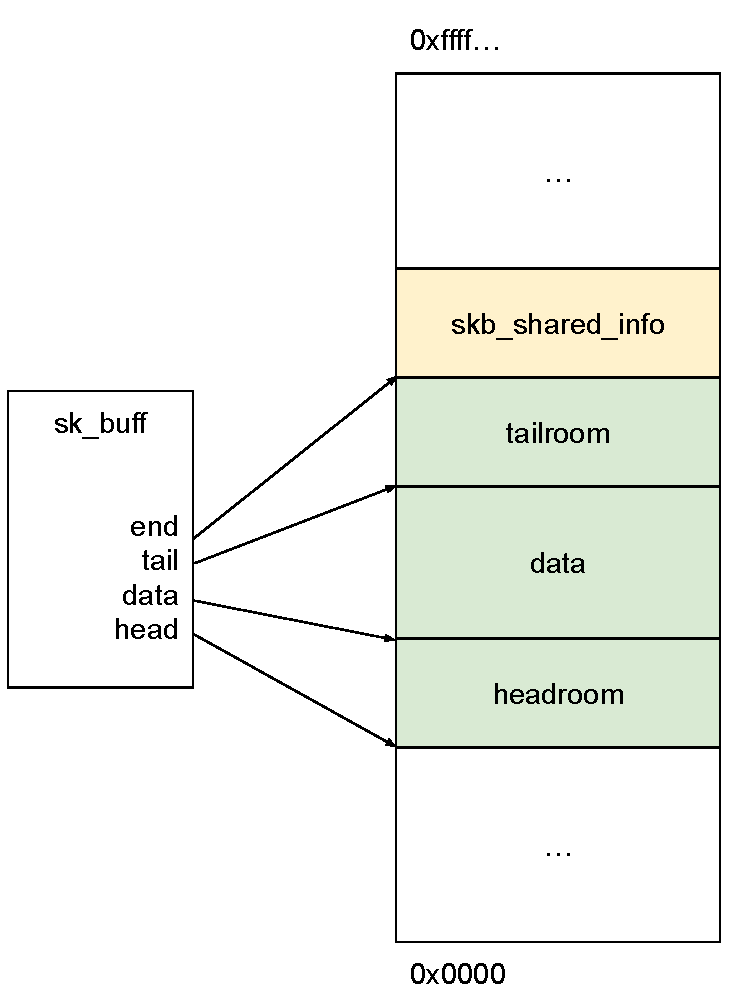
\includegraphics[width=\textwidth]{slides/networking-skb/skb.pdf}
		\end{column}
		\begin{column}{0.7\textwidth}
			\begin{itemize}
				\item \code{skb} maintains positions to the data buffer
				\item The \textbf{data} section is the current \textbf{payload}
				\item The payload boundaries (\code{data} and \code{tail}) depend on the current Layer
				\item \code{skb->len} identifies the current length of data
				\item \code{skb->head} : Start of the allocated buffer
				\item \code{skb->data} : Start of the \textbf{payload section} of the \textbf{current layer}
				\item \code{skb->tail} : End of the payload section
				\item \code{skb->end} : End of the buffer
				\item These pointers are \textbf{moved} when the skb traverses the stack
			\end{itemize}
		\end{column}
	\end{columns}
\end{frame}

\begin{frame}{skb geometry : Paged skb}
	\begin{columns}
		\begin{column}{0.25\textwidth}
			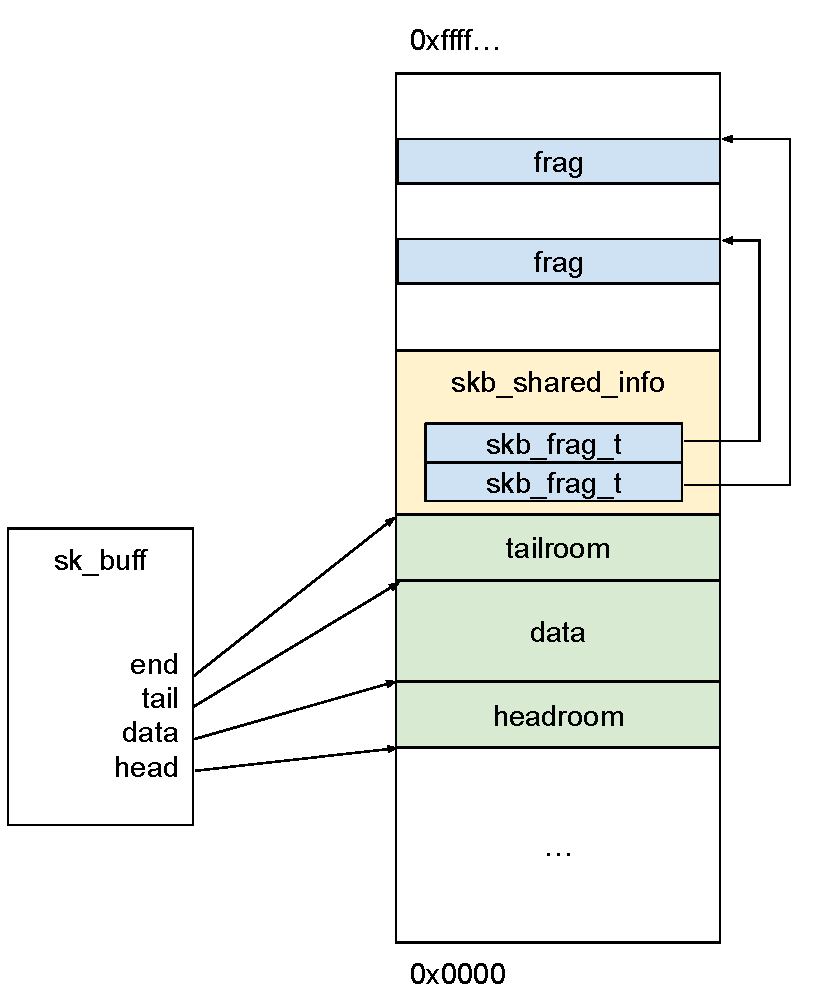
\includegraphics[width=1.3\textwidth]{slides/networking-skb/skb_nonlinear.pdf}
		\end{column}
		\begin{column}{0.75\textwidth}
			\begin{itemize}
				\item The data section of an \code{skb} may be non-contiguous
				\item We talk about \textbf{non-linear} or \textbf{paged} skb.
				\item Sections of the payload are stored in the \code{skb_shared_info}
				\item Each part of the buffer is stored in an array of \code{skb_frag_t}
				\item This happens when transmitting \textbf{scatter-gather} (SG) buffers
				\item \kfunc{skb_linearize} will convert it to a single-buffer skb.
					\begin{itemize}
						\item Useful for drivers that don't support SG.
					\end{itemize}
			\end{itemize}
		\end{column}
	\end{columns}
\end{frame}

\begin{frame}{skb geometry : Fragmented skb}
	\begin{columns}
		\begin{column}{0.3\textwidth}
			% Changme
			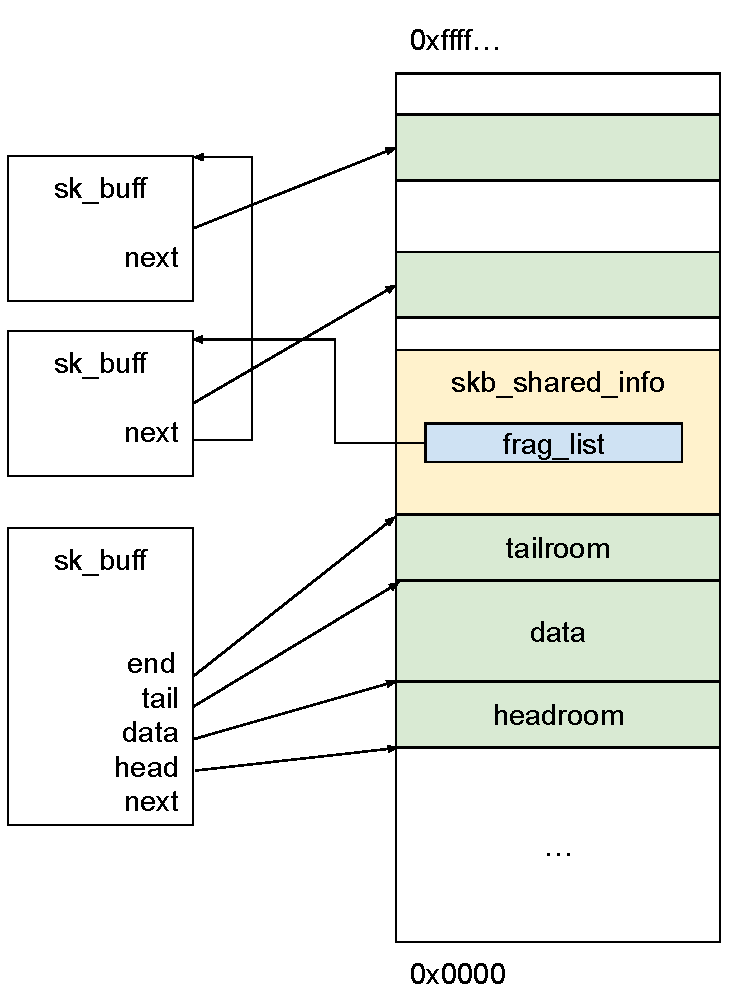
\includegraphics[width=\textwidth]{slides/networking-skb/fragmented_skb.pdf}
		\end{column}
		\begin{column}{0.7\textwidth}
			\begin{itemize}
				\item Buffer bigger than the \textbf{MTU} needs to be fragmented
				\item The original \code{skb} gets split into multiple parts
				\item Each fragment is its \textbf{own skb}
				\item Fragments are chained together through :
					\begin{itemize}
						\item \code{skb_shared_info->frag_list} for the \textbf{first skb}
						\item \code{skb->next} for the other fragments
					\end{itemize}
			\end{itemize}
		\end{column}
	\end{columns}
\end{frame}


\begin{frame}{skb cloning and duplication}
	\begin{columns}
		\begin{column}{0.3\textwidth}
			% Changme
			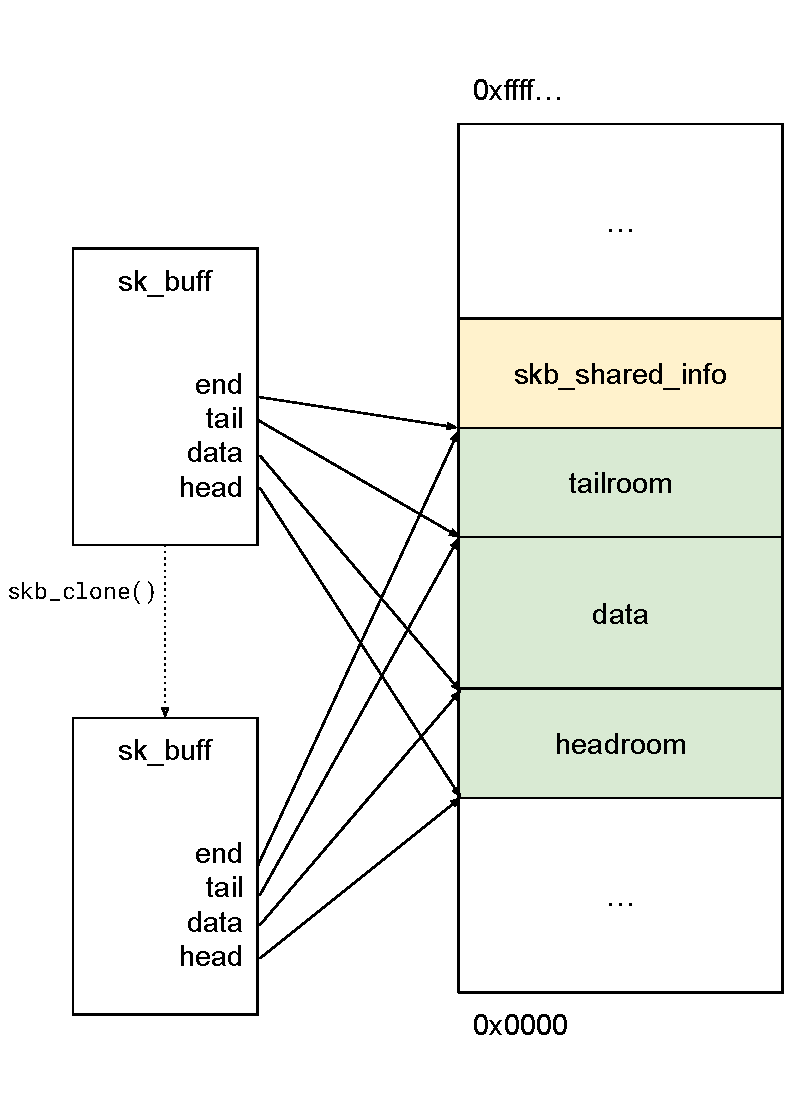
\includegraphics[width=\textwidth]{slides/networking-skb/skb_clone.pdf}
		\end{column}
		\begin{column}{0.7\textwidth}
			\begin{itemize}
				\item \kfunc{skb_clone} allocates a new \kstruct{sk_buff} pointing to an existing buffer
				\item Useful when the \code{skb} needs to be delivered multiple times
					\begin{itemize}
						\item For Multicast, \code{AF_PACKET}, capturing, etc.
					\end{itemize}
				\item The fragments are also cloned
				\item The buffer memory is \textbf{refcounted}
				\item Destroy the clone with \kfunc{consume_skb} or \kfunc{kfree_skb}
				\item \kfunc{skb_copy} duplicates the \code{skb} and all its associated memory
				\item \kfunc{pskb_copy} duplicates the \code{skb} and the \textbf{header} but clones the payload
				\item \code{skb} can also be shared, tracked with \code{skb->shared}
			\end{itemize}
		\end{column}
	\end{columns}
\end{frame}

\begin{frame}{skb layer offsets}
	\begin{columns}
		\begin{column}{0.3\textwidth}
			% Changme
			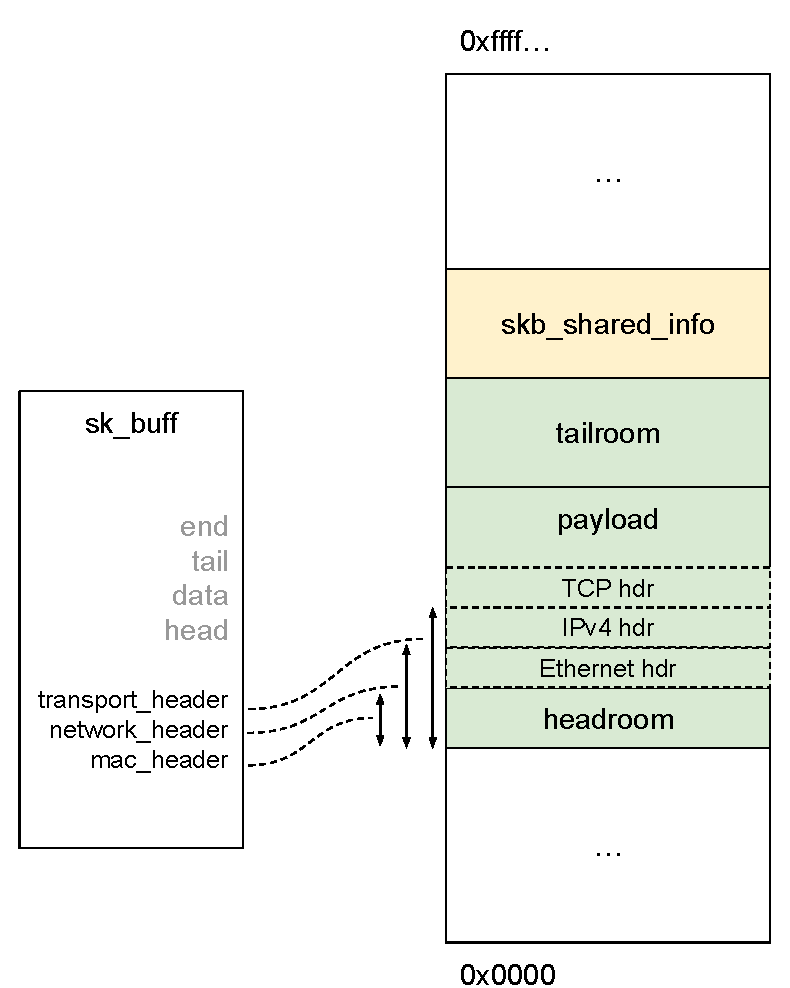
\includegraphics[width=\textwidth]{slides/networking-skb/skb_layers_offsets.pdf}
		\end{column}
		\begin{column}{0.7\textwidth}
			\begin{itemize}
				\item \kstruct{sk_buff} maintains \textbf{layer offsets} starting from \code{skb->head}
				\item Set and modified by each encapsulation or decapsulation step
				\item When processing a packet, each layer moves \code{skb->data}
				\item \code{skb_reset_xxx_header()} sets the given header \textbf{where \code{skb->data} currently is}
					\begin{itemize}
						\item \kfunc{skb_reset_mac_header} : Called by \textbf{drivers}
						\item \kfunc{skb_reset_network_header} : Called after MAC processing
						\item \kfunc{skb_reset_transport_header} : Called in L3 (IP) processing
					\end{itemize}
			\end{itemize}
		\end{column}
	\end{columns}
\end{frame}

\begin{frame}{\kfunc{skb_pull}}
	\begin{columns}
		\begin{column}{0.4\textwidth}
			% Changme
			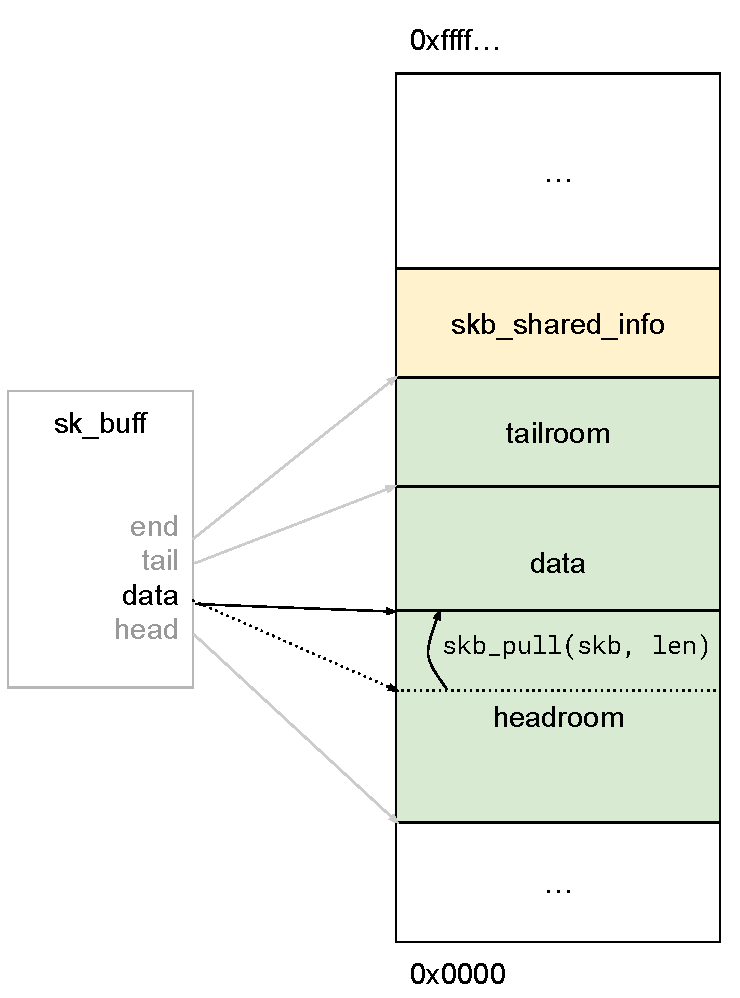
\includegraphics[width=\textwidth]{slides/networking-skb/skb_pull.pdf}
		\end{column}
		\begin{column}{0.6\textwidth}
			\begin{itemize}
				\item Pulls header data, used during \textbf{decapsulation}
				\item Decreases \code{skb->len}
				\item Usually followed by a layer offset readjustment
				\item Returns the new \code{skb->data} pointer
				\item May fail if \code{skb->len} is too short
				\item May require a \textbf{checksum recompute}
					\begin{itemize}
						\item \kfunc{skb_pull_rcsum} will update checksums
					\end{itemize}
			\end{itemize}
		\end{column}
	\end{columns}
\end{frame}

\begin{frame}{\kfunc{skb_push}}
	\begin{columns}
		\begin{column}{0.4\textwidth}
			% Changme
			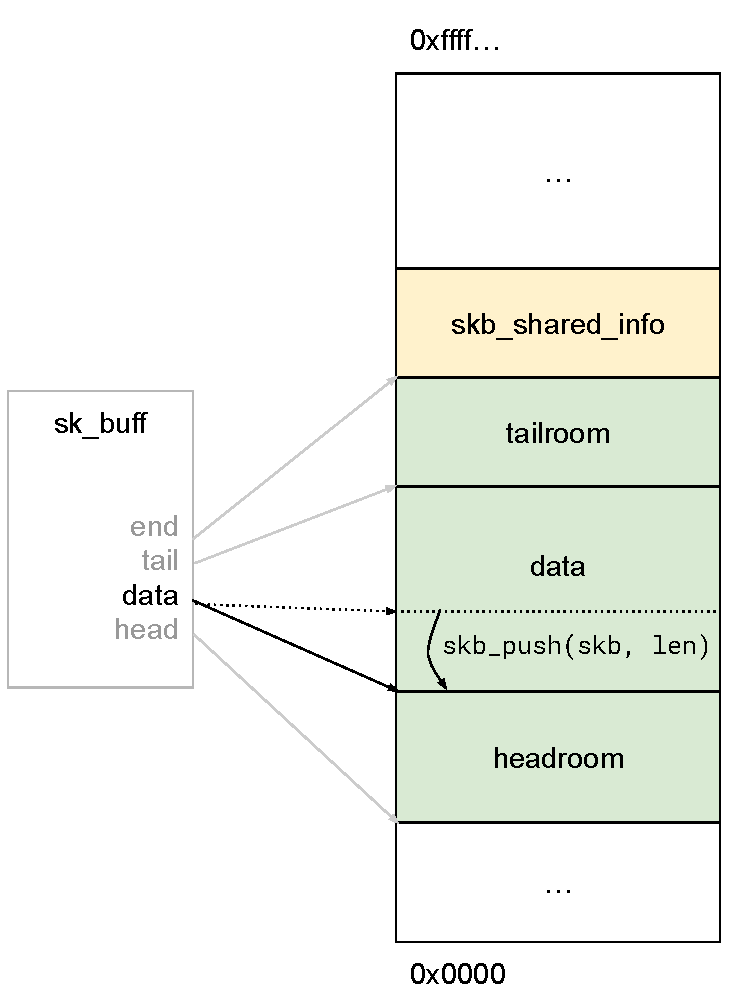
\includegraphics[width=\textwidth]{slides/networking-skb/skb_push.pdf}
		\end{column}
		\begin{column}{0.6\textwidth}
			\begin{itemize}
				\item Pushes the \code{skb->data} into the headroom
				\item Increases \code{skb->len}
				\item Used during \textbf{encapsulation}, when creating the headers
				\item May fail if the headroom is too short
				\item May require a \textbf{checksum recompute}
					\begin{itemize}
						\item \kfunc{skb_push_rcsum} will update checksums
					\end{itemize}

			\end{itemize}
		\end{column}
	\end{columns}
\end{frame}

\begin{frame}{\kfunc{skb_put}}
	\begin{columns}
		\begin{column}{0.4\textwidth}
			% Changme
			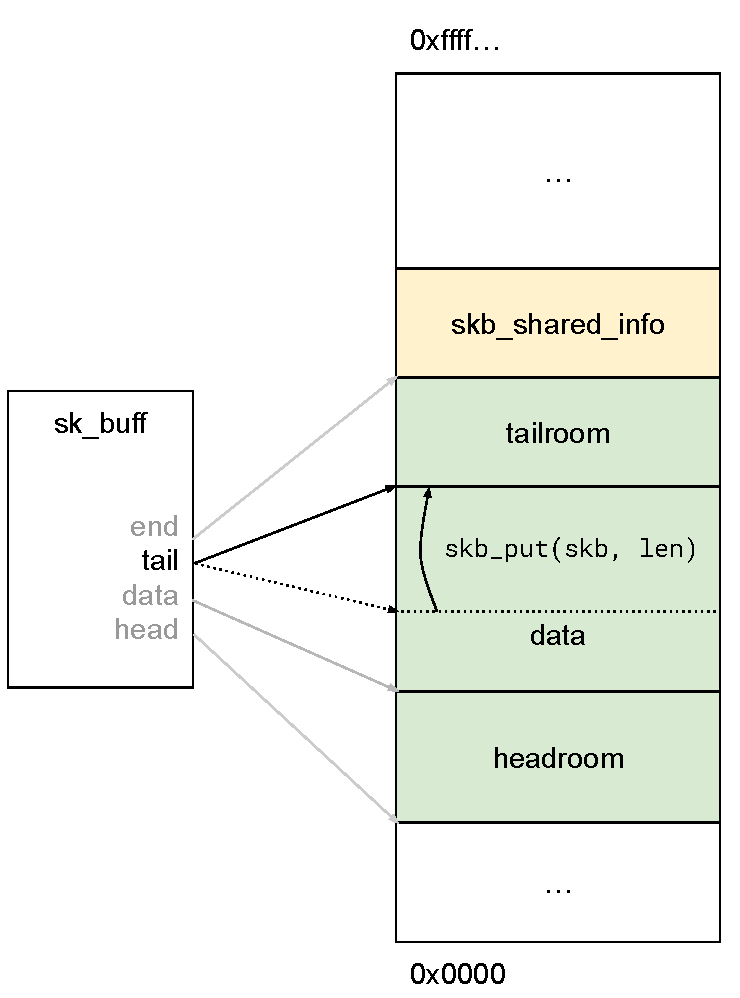
\includegraphics[width=\textwidth]{slides/networking-skb/skb_put.pdf}
		\end{column}
		\begin{column}{0.6\textwidth}
			\begin{itemize}
				\item Expands the payload section into the tailroom
				\item Increases \code{skb->len}
				\item Used in drivers to set the \textbf{full packet size}
				\item Also used by some \textbf{DSA taggers}
			\end{itemize}
		\end{column}
	\end{columns}
\end{frame}

\begin{frame}{\kfunc{skb_trim}}
	\begin{columns}
		\begin{column}{0.4\textwidth}
			% Changme
			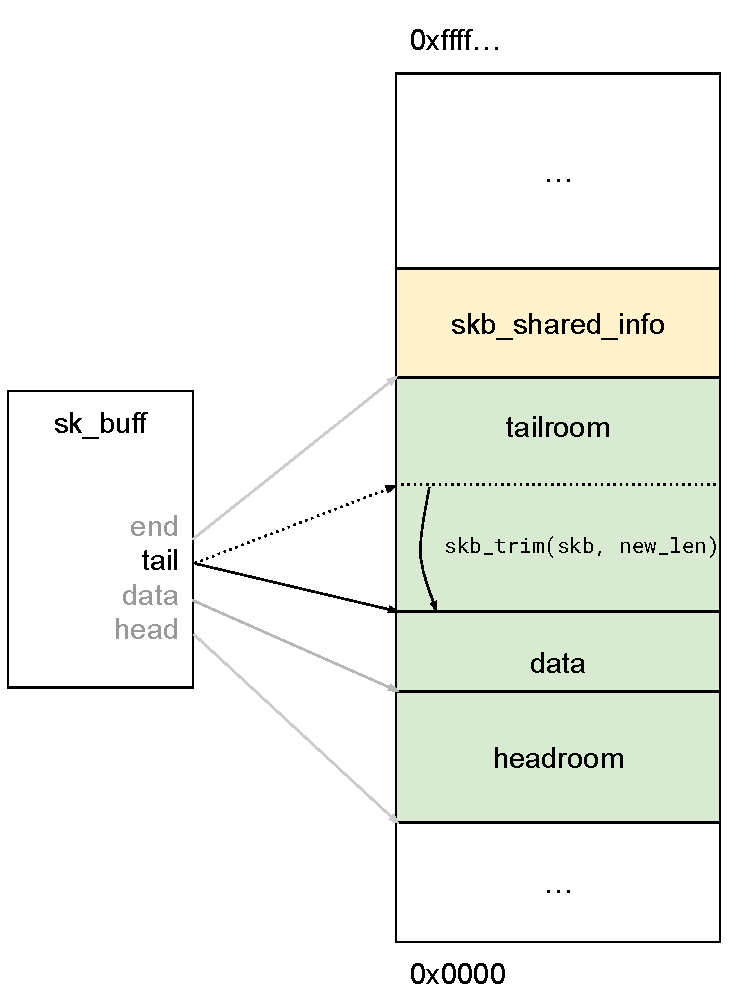
\includegraphics[width=\textwidth]{slides/networking-skb/skb_trim.pdf}
		\end{column}
		\begin{column}{0.6\textwidth}
			\begin{itemize}
				\item Shrinks down the payload from its end
				\item Decreases \code{skb->len}
				\item Only works on \textbf{linear skb}
				\item Used to remove padding
				\item Also useful to decapsulate protocols that insert a trailer
					\begin{itemize}
						\item e.g. \href{https://elixir.bootlin.com/linux/v6.15.1/source/net/hsr/hsr_forward.c\#L196}{PRP}
					\end{itemize}
			\end{itemize}
		\end{column}
	\end{columns}

\end{frame}

\begin{frame}{pskb helpers}
	\begin{itemize}
		\item \textbf{p}otentially fragmented \textbf{skb} helpers manipulate non-linear \code{skb}
		\item Useful if you don't know and don't mind if the \code{skb} is paged
		\item Not all helpers have a matching \code{pskb} equivalent, not always relevant
		\item \kfunc{skb_put} => \kfunc{pskb_put}
		\item \kfunc{skb_pull} => \kfunc{pskb_pull}
		\item \kfunc{skb_trim} => \kfunc{pskb_trim}
		\item \kfunc{pskb_may_pull} indicates if a \code{pskb_pull} operation will succeed
			\begin{itemize}
				\item \kfunc{pskb_may_pull_reason} returns a \textbf{drop reason} if it will fail
			\end{itemize}
	\end{itemize}
\end{frame}

\begin{frame}{skb allocation}
	\begin{itemize}
		\item \kfunc{build_skb} allocates a new \code{skb} around an existing buffer
		\item A new linear \code{skb} is allocated with \kfunc{alloc_skb}. It also allocates its data buffer.
		\item A paged \code{skb} can be allocated with \kfunc{alloc_skb_with_frags}
		\item A newly-allocated \code{skb} is empty : \code{skb->data} == \code{skb->head} == \code{skb->tail}
		\item \kfunc{skb_reserve} grows the headroom, then \kfunc{skb_push} to prepare the data section
	\end{itemize}
	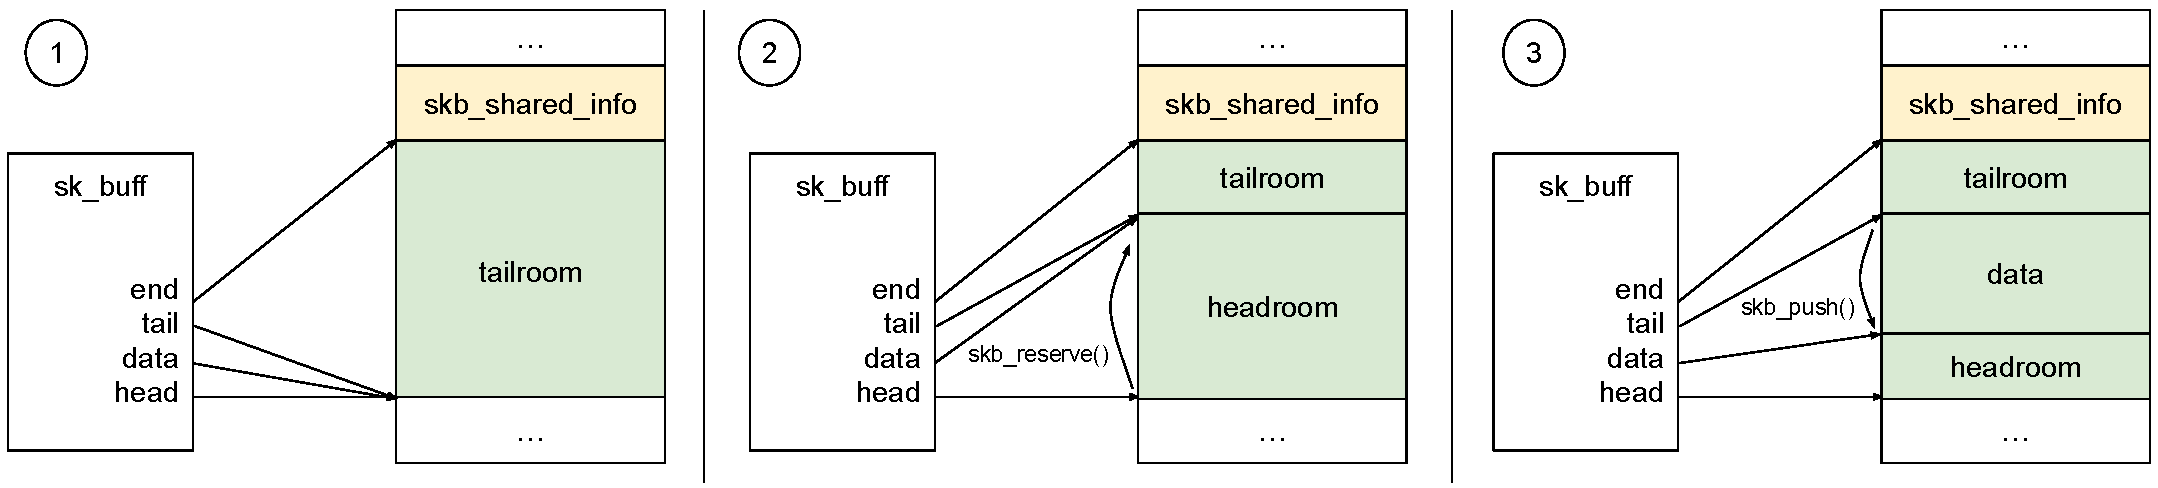
\includegraphics[width=\textwidth]{slides/networking-skb/newskb.pdf}
\end{frame}

\begin{frame}[fragile]{Dropping packets}
	\begin{itemize}
		\item At any point, we may decide to \textbf{discard} an \code{skb}, it is \textbf{dropped}
		\item an \code{skb} is dropped with : \\
		\begin{minted}{c}
void kfree_skb_reason(struct sk_buff *skb, enum skb_drop_reason reason);
		\end{minted}
	\item The \code{reason} allows reporting to users the cause of the drop
	\item Around 120 different reasons currently exist
		\begin{itemize}
			\item see \kfile{include/net/dropreason-core.h}
		\end{itemize}
	\item Drop reasons are not part of the \textbf{userspace API}, but can be retrieved with :
		\begin{itemize}
			\item \textbf{ftrace}, via the \code{skb:kfree_skb} and \code{skb:consume_skb}tracepoints : \\
				\code{trace-cmd record -e skb:kfree_skb <cmd>}
			\item \textbf{dropwatch} : Uses the kernel's \code{dropmon} mechanism through \code{netlink}
			\item \textbf{retis} : \code{eBPF}-based, uses the \code{BTF} information to display reasons
		\end{itemize}
	\end{itemize}
\end{frame}

\begin{frame}{SKB decapsulation}
	\begin{columns}
		\column{0.3\textwidth}
		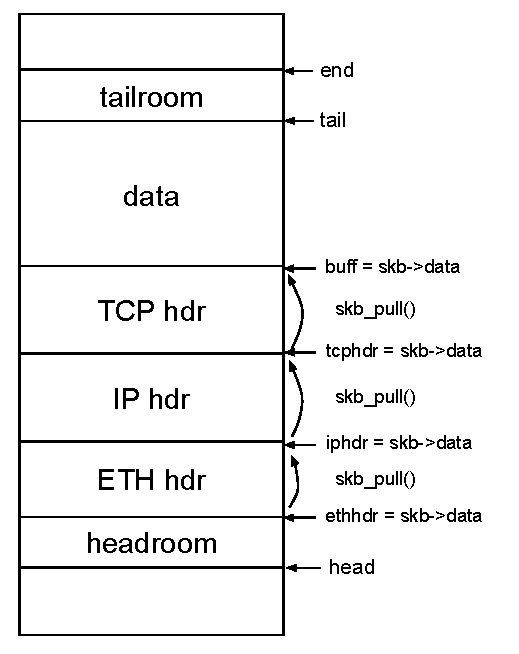
\includegraphics[width=1.2\textwidth]{slides/networking-skb/skb_decapsulation.pdf}
		\column{0.7\textwidth}
		\begin{itemize}
			\item When \textbf{ingress} packets traverse the stack, they are decapsulated
			\item Each header usually has a field indicating the nature of the upper layer
				\begin{itemize}
					\item Ethernet header : \code{Ethertype} (2 bytes)
					\item IPv4 header : \code{Protocol} (1 byte)
					\item IPv6 header : \code{Next Header} (1 byte)
				\end{itemize}
			\item The \code{ptype} list maps \code{Ethertypes} to \code{packet handlers}
			\item The \code{proto} list maps \code{Protocols} to \code{Transport handlers}
			\item Each stage \textbf{parses} its header, and \textbf{moves \code{skb->data}}
			\item In the last stage, \code{skb->data} points to the final payload
		\end{itemize}
	\end{columns}
\end{frame}

\begin{frame}[fragile]{\kstruct{packet_type}}
	\begin{itemize}
		\item L2 protocols such as \code{802.3} and \code{802.11} usually include an \textbf{Ethertype}
		\item 2-byte value indicating the higher-level protocol :
			\begin{itemize}
				\item \code{0x0800} for IPv4, \code{0x0806} for ARP
				\item \code{0x86dd} for IPv6, \code{0x8100} for 802.1Q (vlan)
				\item See \kfile{include/uapi/linux/if_ether.h}
			\end{itemize}
		\item We can associate \kstruct{packet_type} with Ethertypes : \\
			\begin{minted}{c}
struct packet_type {
    __be16 type;
    struct net_device *dev;
    int (*func) (struct sk_buff *skb,
                 struct net_device *dev,
                 struct packet_type *ptype,
                 struct net_device *orig_dev);
    /* ... truncated */
};
			\end{minted}
	\end{itemize}
\end{frame}

\begin{frame}[fragile]{\kfunc{dev_add_pack}}
	\begin{itemize}
		\item \kfunc{dev_add_pack} registers a \kstruct{packet_type} (\code{ptype})
		\item if \code{ptype->dev} is \code{NULL}, the handler is registered system-wide
			\begin{itemize}
				\item e.g. IPv4, IPv6, ARP
			\end{itemize}
		\item otherwise, the \code{ptype} will only be handled on \code{ptype->dev}.
			\begin{itemize}
				\item e.g. \code{AF_PACKET} sockets bound to an interface
			\end{itemize}
		\item Upon match of the Ethertype, \code{ptype->func()} is called with the \code{skb}
		\item \code{ptype->list_func} can be implemented to handle multiple \code{skb}
	\end{itemize}
\end{frame}

\begin{frame}[fragile]{IPv4 example}
	\begin{minted}{c}
static struct packet_type ip_packet_type __read_mostly = {
        .type = cpu_to_be16(ETH_P_IP),
        .func = ip_rcv,
        .list_func = ip_list_rcv,
};

static int __init inet_init(void) /* truncated */
{
        /* For TX : Used by the socket's sendmsg */
        proto_register(&tcp_prot, 1);
        proto_register(&udp_prot, 1);
        proto_register(&ping_prot, 1);

        /* For RX : Handle the IP Ethertype */
        dev_add_pack(&ip_packet_type);
}
	\end{minted}
\end{frame}

\begin{frame}{Exception : Vlan}
	\begin{itemize}
		\item VLANs (802.1Q and 802.1AD) have a dedicated Ethertype, but no \kstruct{packet_type}
		\item VLANS are handled \href{https://elixir.bootlin.com/linux/v6.15.1/source/net/core/dev.c\#L5756}{directly in the receive path}
		\item Some hardware can strip the VLAN tag themselves
			\begin{itemize}
				\item The tag is reported out-of-band, such as \href{https://elixir.bootlin.com/linux/v6.15.1/source/drivers/net/ethernet/freescale/enetc/enetc.c\#L1363}{in the DMA descriptors}
				\item The VLAN information is set in \code{skb->vlan_proto} and \code{skb->vlan_tci}
			\end{itemize}
		\item This also allows optimizing speed by avoiding indirect branches
		\item Some hardware may also perform \href{https://elixir.bootlin.com/linux/v6.15.1/source/drivers/net/ethernet/marvell/mvpp2/mvpp2_main.c\#L5295}{Vlan filtering}
	\end{itemize}
\end{frame}

\begin{frame}[fragile]{RX handlers}
	\begin{itemize}
		\item Protocol information alone may not always be sufficient for custom processing
		\item e.g. \textbf{MACVlan} has no dedicated Ethertype
		\item We can attach a callback function to a netdev, executed before protocol handling \\
			\begin{minted}{c}
rx_handler_result_t rx_handler_func_t(struct sk_buff **pskb);
			\end{minted}
		\item Attached with \kfunc{netdev_rx_handler_register} (One handler per netdev)
		\item Handler may change the \code{skb}, including \code{skb->dev}, and return :
			\begin{itemize}
				\item \code{RX_HANDLER_CONSUMED} : \code{skb}'s processing stops here
				\item \code{RX_HANDLER_PASS} : continue as if the handler didn't exist
				\item \code{RX_HANDLER_EXACT} : \code{PASS} to protocol only if \code{ptype->dev == skb->dev}
				\item \code{RX_HANDLER_ANOTHER} : Re-process the \code{skb} as if it came from \code{skb->dev}
			\end{itemize}
	\end{itemize}
\end{frame}

\begin{frame}[fragile]{\kstruct{net_protocol}}
	\begin{itemize}
		\item Layer 3 protocols include an 8-bit identifier describing the L4 layer
			\begin{itemize}
				\item \code{6} for TCP, \code{17} for UDP
				\item \code{1} for ICMP, \code{41} for IPv6-in-IPv4
				\item see \kfile{include/uapi/linux/in.h}
			\end{itemize}
		\item A \textbf{transport protocol handler} is represented by \kstruct{net_protocol}
			\begin{itemize}
				\item For IPv6, it is represented by \kstruct{inet6_protocol}
			\end{itemize}
	\end{itemize}
	\begin{minted}{c}
struct net_protocol {
        int (*handler)(struct sk_buff *skb);
        int (*err_handler)(struct sk_buff *skb, u32 info);
        ...
};

	\end{minted}
\end{frame}

\begin{frame}[fragile]{\kfunc{inet_add_protocol} and \kfunc{inet6_add_protocol}}
	\begin{itemize}
		\item Transport protocols are registered in each L3 stack
		\item \begin{minted}{c}
int inet_add_protocol(struct net_protocol *prot, u8 num);
		\end{minted}
		\item \begin{minted}{c}
int inet6_add_protocol(struct inet6_protocol *prot, u8 num);
		\end{minted}
	\item Associate protocols with their respective identifiers
	\item Upon matching the \code{num} identifier, \code{prot->handler()} is called

	\end{itemize}
\end{frame}

\begin{frame}[fragile]{\kstruct{net_offload}}
	\begin{itemize}
		\item Some Layer 4 protocols may be associated with a \kstruct{net_offload}
		\item Used to offload \textbf{segmentation} : Let the hardware or driver do it
			\begin{itemize}
				\item Segmentation and re-assembly is protocol-specific
				\item Each protocol can register a \kstruct{net_offload}
				\item \begin{minted}{c}
int inet_add_offload(const struct net_offload *prot, unsigned char num);
int inet6_add_offload(const struct net_offload *prot, unsigned char num);
				\end{minted}
			\end{itemize}
		\item \code{skb}s bigger than the \textbf{MTU} are passed to the driver
		\item The driver or the hardware handles splitting the packet
			\begin{itemize}
				\item L2 and L3 headers are added, and a shorter L4 header
			\end{itemize}
		\item On the receive side, the hardware or driver re-assembles the packets
			\begin{itemize}
				\item Intermediate headers are stripped and the packet is re-assembled
			\end{itemize}
	\end{itemize}
\end{frame}

\begin{frame}{Generic Receive Offload}
	\begin{itemize}
		\item GRO may be used if the driver or the hardware doesn't handle re-assembly
			\begin{itemize}
				\item May be toggled with \code{ethtool -K <iface> gro off|on}
			\end{itemize}
		\item It is \textbf{generic}, works with any Layer 4 protocol
		\item This still requires driver support :
			\begin{itemize}
				\item Upon receiving packets, fragmented or not, call \kfunc{napi_gro_receive}
				\item Drivers that do not support it call \kfunc{netif_receive_skb}
			\end{itemize}
		\item GRO accumulates \code{skbs} and asks L3 and L4 to act upon it
			\begin{itemize}
				\item \kfunc{inet_gro_receive} : e.g. Checks if Don't Fragment flag is set
				\item \kfunc{tcp_gro_receive} : e.g. Flush if we exceed the TCP MSS
			\end{itemize}
		\item GRO-held \code{skb}s are merged and eventually flushed to the regular receive path
		\item Can be problematic for latency or throughput in \textbf{router} mode
	\end{itemize}
\end{frame}

\begin{frame}{Generic Segmentation Offload}
	\begin{itemize}
		\item Perform the segmentation either in hardware, or just before passing to the driver
		\item Avoids having all the segments traverse the stack
			\begin{itemize}
				\item Routing, filtering, scheduling decisions are the same for all segments
			\end{itemize}
		\item Pure software implementation, but can be offloaded to hardware :
			\begin{itemize}
				\item TCP Segmentation Offload (TSO)
				\item Hardware will split the TCP data based on the MSS
				\item Support for partial checksum offload is required
			\end{itemize}
	\end{itemize}
\end{frame}

\begin{frame}{routing}
	\begin{columns}
		\column{0.4\textwidth}
		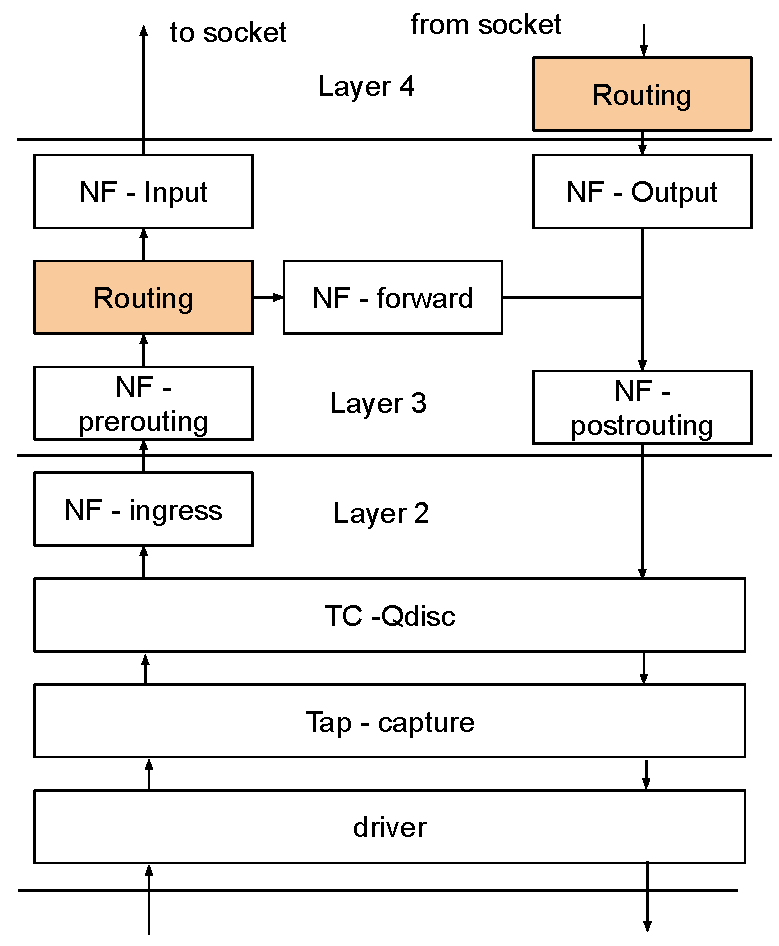
\includegraphics[width=1\textwidth]{slides/networking-skb/routing.pdf}
		\column{0.6\textwidth}
		\begin{itemize}
			\item Routing happens on \textbf{ingress} and \textbf{egress}
			\item Done by looking-up the \textbf{F}orwarding \textbf{I}nformation \textbf{B}ase
			\item Decision taken in \kfunc{fib_lookup}
			\item The table can be shown with \textbf{ip route}
		\end{itemize}
	\end{columns}
\end{frame}

% important internal stuff
% Lifetime, drop and reasons
% cloning vs dup
% packet_add, proto and stack traversal
\begin{frame}{Flow tables}
	\begin{itemize}
		\item Allows a slow-path and fast-path for routing and bridging
		\item The first packet of a given flow goes through the whole stack
		\item The final routing or bridging decision is cached
		\item The next packet from the same flow will go through the fast-path
		\item These decisions may be offloaded to hardware
	\end{itemize}
\end{frame}


